\documentclass[runningheads,a4paper]{llncs}
\usepackage{amssymb}
\setcounter{tocdepth}{3}
\usepackage{graphicx}

\pagestyle{empty}
\begin{document}

\mainmatter  

\title{The Use of k-means Algorithm to Improve\\Kernel Method via Instance
		Selection}

\titlerunning{Use k-means Algorithm to Improve Kernel Method}

\author{Lulu Wang}

\authorrunning{Lulu Wang}

\institute{Department of Computer Science and Technology,\\
		JiLin University, 130012 ChangChun, China\\
		\url{naruto7@icloud.com}}

\toctitle{Lecture Notes in Computer Science}
\tocauthor{Authors' Instructions}

\maketitle



\begin{abstract}
		The kernel method is well known for its success in solving the
		curse of dimension of linearly inseparable problems. But as an instance-
		based learning algorithm it suffers from high memory requirement and
		low efficiency in that it needs to store all of the training instances. And
		when there are noisy instances classification accuracy can suffer. In this
		paper we present an approach to alleviate both of the problems mentioned
		above by using $k$-means algorithm to select only $k$ representativeness
		instances of the training data. And we view the selected $k$ instances
		as the new data set, where the choice of the value of $k$ is influenced
		by the size and the character of the data set. It turn out
		that with a carefully selected $k$ we can still get a good performance
		while the number of the instances stored are greatly decreased.


\keywords{$k$-means; instance selection; kernel method}
\end{abstract}


\section{Introduction}
		There are mainly two kinds of problems in supervised learning: regression problem
 		and classification problem, and until now we have many successful algorithms
		to solve different kinds of problems \cite{jour1}. These algorithms can be
		classified into two kinds, one of which is parameter-based learning algorithm
		and the other is instance-based learning algorithm.

		For the parameter-based learning algorithm, we use the training instances to
		train our model, usually by applying some methods (such as gradient descent)
		to change the parameter of the model until reaching a local or global minima
		of the cost function, and then we get the target parameter of the model.
		After that we don not need the instance any more so the model is
		light and of lower cost in predicting the value or the class of a new instance. And
		by now, most of the supervised learning algorithm is parameter-based (such as
		logistic regression, decision tree and so on).

		However, there are some algorithms that are instance-based which means that
		the algorithm need to store all of the training instances and use these instances
		to predict a new input. Unfortunately these algorithms are limited by its high
		requirement for memory and low speed in computation especially in large scale
		problem \cite{jour3}. And the kernel method is one of the instance-based approach.

		The kernel method is successfully used in some learning algorithms such as SVM, 
		however it also suffers from the problems mentioned above.
		Motivated by that we study how to improve the kernel method and in this paper
		we provide a simple way to achieve this goal. We use the $k$-means algorithm to 
		select just a small part of the instances to train the model. We run the 
		$k$-means algorithm on our training
		set and separate the training set into $k$ parts, then we make a statistic on the
		label of the instances in every part individually and use the cluster centroid as a 
		new instance and the most appeared label in that cluster as its label, then
		we get the new training set with only $k$ instances.
		And since the new training set is much smaller, the algorithm do not need as much
		memory as before and can also run much faster. While running the $k$-means we
		have ignored the noisy instances in choosing the new label and the new instance
		thus this approach will also increase the robustness of the kernel method.

		There is still a problem before we can run the $k$-means algorithm, that is
		the choice of $k$. Intuitively, the larger the $k$ is the
		more accuracy the result is but the more memory and time the algorithm needs,
		because in running the $k$-means algorithm we will lose some information of the
		data set which will result in the decrease of the accuracy. So we need to get
		a compromise between the accuracy and the cost of the algorithm. In practice
		(just as how we choose a proper dimension when we use PCA to decrease the
		dimension of our data), we can choose a $k$ that decrease the accuracy within our
		tolerance (for example 1\% loss of the accuracy or even 5\% loss of the accuracy).

\section{Problem Formalism}
	 	In supervised learning problem, we are given a set of labeled training data of $m$
		instances $\{(x^{(i)}, y^{(i)})|i = 1, 2, 3, ...,m\}$. Here each $x^{(i)}$ $\in$ $R^{n}$ is an n dimensional
		feature vector, for classification problem, $y^{(i)}$ $\in$ $\{1,2,..., C\}$ is the corresponding
 		class label (for regression problem $y^{(i)}$ $\in$ $R$). In general kernel method
		algorithm we need all of the $m$ instance, but here we will use the $k$-means algorithm
 		to select only $k$ new instances $\{(x^{(i)}_n, y^{(i)}_n)|i = 1, 2, 3, ...,k\}$
		(the subscript $n$ indicates that it is a instance from the new data set) to replace
		the $m$ original set and here $k$ should be smaller than $m$. Finally we use this new
		data set to train our model.

\section{Algorithm}
		Kernel method can be used in many different models, such as SVM, logistic
		regression, etc.in this paper we describe just
		one example of how to use the algorithm. We will use the Gaussian kernel SVM as our 
		training model to demonstrate our method.

\subsection{Instance Selection}

		In this section, we will give the detail steps of how to get the labeled data set
		$\{(x^{(i)}_n, y^{(i)}_n)|i = 1, 2, 3, ...,k\}$ from the larger original data set 
		$\{(x^{(i)}, y^{(i)})|i = 1, 2, 3, ...,m\}$. 
		We will apply $k$-means to finish this task, and we will use the Euclidian distance to describe the similarity
		between two instances. Before we run the $k$-means algorithm
		we need to choose different value of $k$. And then we need
		to randomly choose $k$ instances from the original data set $\{x^{(1)},x^{(2)},..., x^{(m)}\}$
		(here we temporally ignore the label of each $x^{(i)}$) as the initial value of the
		$k$ centroids $\{x^{(1)}_n, x^{(2)}_n,..., x^{(k)}_n\}$. After that we run the $k$-means algorithm
		until the partition of the data set dose not change. After that, we got $k$ clusters of instances and $k$ centroids
		$\{x^{(1)}_n, x^{(2)}_n,..., x^{(k)}_n\}$. Then use the label appears most in a cluster 
		as the label for the corresponding centroid, and view the $k$ centroids 
		and its label as the new training set of the problem.

\subsection{Training the model}

		Kernel SVM is a variation of SVM. SVM is well known for its good property: it can create
		a hyperplane with a maximum margin between different labeled data set. In some cases when the data set is linearly 
		inseparable we need to project the input feature to a higher dimensional feature in Hilbert space. However as the
		dimension of the input feature increases the dimension of the projected feature will increase exponentially. Under this 
		case, we can use the kernel SVM to solve this problem. Generally, kernel SVM is a linear combination of the kernel 
		function $\sigma(x,x^{(i)})$ for each input $x^{(i)}$. It successfully solved the dimensional explosion, but there also exist
		some drawbacks as we have already mentioned. In our previous work we get a training set with much smaller number of instances 
		than the original big one, and use it to train our kernel SVM. Now we will give the following algorithm to illustrate the whole process.


\medskip
\noindent
{\it Algorithm: instance selection and model training}
\begin{verbatim}
	Input: The original data set x[1]...x[n], y[1]...y[n] and k.
		1. Running the k-means algorithm to get k clusters from 
		   the original training set.
		2. Label each cluster with the mostly appeared label 
		   in that cluster.
		3. Construct a new instance set nx[1]...nx[k], 
		   ny[1]...ny[k], use the k clusters centroid and its label.
		4. Use the new instance to train a kernel SVM.
	Output: A improved kernel SVM. 
	
\end{verbatim}
\medskip


\subsection{Experiments}

		In our experiments we trained a SVM with Gaussion kernel:
		\[
			K(x,z)=\exp(- \frac{{{{\left\| {x - z} \right\|}^2}}}{{2{\sigma ^2}}})
		\]
		and we set the standard SVM regularization    
		parameter $C=1$, and $\sigma=0.1$. We apply the model to two learning tasks: 
		A small data set \footnote{This data set comes from 
		the experiment of Andrew Ng’s Machine learning class.}
		and The Skin Segmentation Data Set \footnote{This data set comes from: \url{archive.ics.uci.edu/
		ml/datasets/Skin+Segmentation} but we only use a part of it}
		which was shown in Table 1. We did the experiments in a computer with a 2.5GHz Intel Core i5 CPU,
		a 4GB 1600 MHz memory and the operation system is MacOS.    

\begin{table}[tbp]
\centering  
\begin{tabular}{c|c|c|c|c}
\hline
		data set &attributes &training set size &test set size &classes\\ 
\hline  
		A small data set &2 &2589 &500 &2\\        
		Skin Segmentation Data Set &3 &24500 &4500 &2\\       
\hline
\end{tabular}
\caption{The description of the data set used for the experiment.}
\end{table}

\begin{table}[tbp]
\centering  
\begin{tabular}{c|c|c|c|c}
\hline
		the value of $k$ &$k=m$ &$k=0.2*m$ &$k=0.1*m$ &$k=0.05*m$\\ 
\hline  
		accuracy of test set &96.93\% &95.92\% &\textbf{95.85\%} &93.93\%\\  
		
		training time & 37.82s &3.46s &\textbf{2.09s} & 0.74s \\
		
		memory requirements  & 60.68kb & 12.14kb & \textbf{6.07kb} & 3.05kb \\     
\hline
\end{tabular}
\caption{The result of the first experiment when $k=m, k=0.2m, k=0.1m$ and $k=0.05m$.}
\end{table}

		In the following two experiments we use the Gaussian kernel SVM as our classifier (the detail of 
		the parameters are mentioned above), and to make the 
		result more intuitionist, we choose the small data set as our first task which has only two 
		attributes and two classes. We choose different $k$ ($k=m$,$k=0.2m$, $k=0.1m$ and $k=0.05m$) when we 
		running the $k$-means algorithm to get our new instances, and we plotted the new data sets for 
		different $k$ as well 
		as the original dataset in Fig.1. According to the result, we can find that the $k$-means algorithm 
		works with good performance in generating the new data set, and intuitively we can find that
		the distribution of 
		the new data set is almost the same with the original data set, thus we can assume that the new data 
		set can also work well in 
		training our model as the original data set. To prove this hypothesis we trained 
		a Gaussian kernel SVM for each new data set as well as the original data set and the result was shown in 
		Table 2. We can learning from the result that we can still get a accuracy of 95.85\% with only 10 percent of 
		the size of the original data set when we choose $k=0.1m$.
		
\begin{figure}[tbp]
\centering

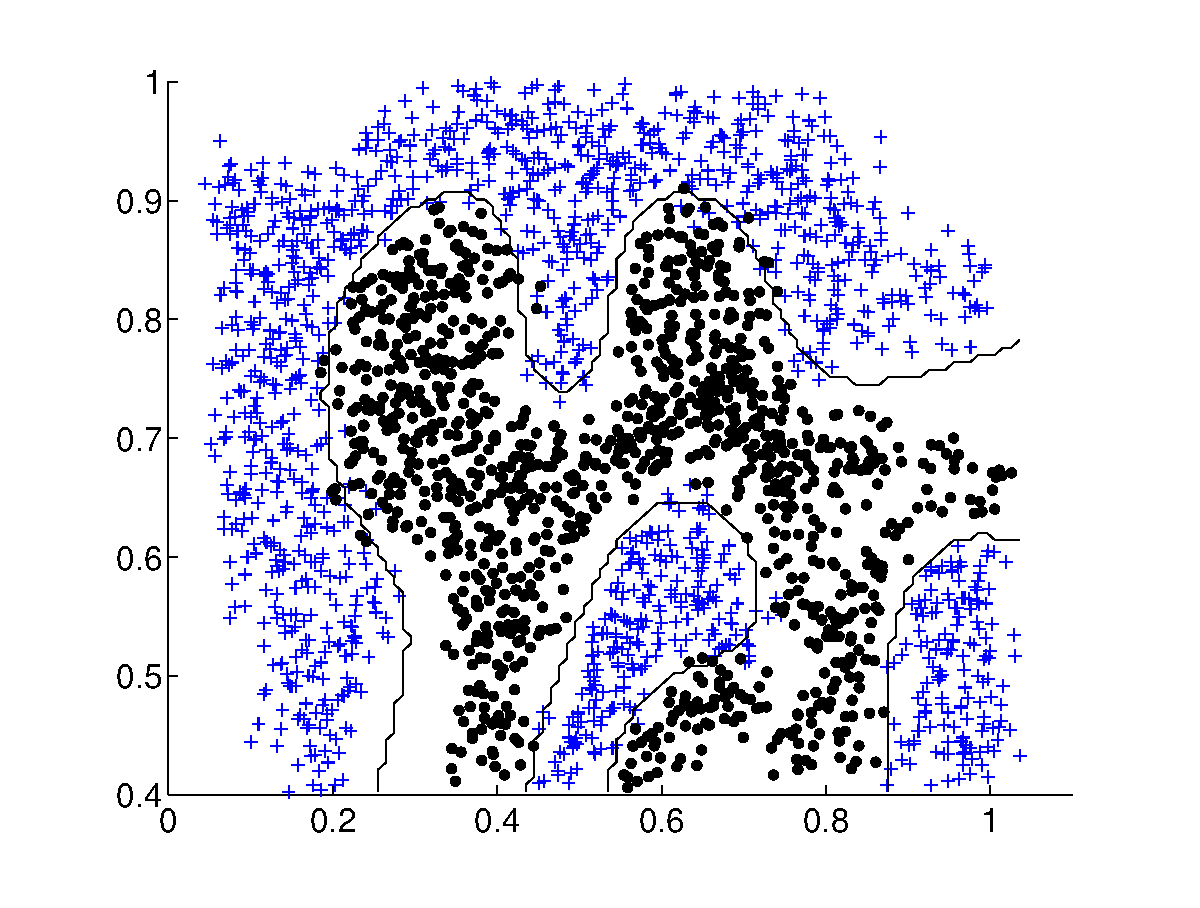
\includegraphics[height=4cm]{a1.eps}
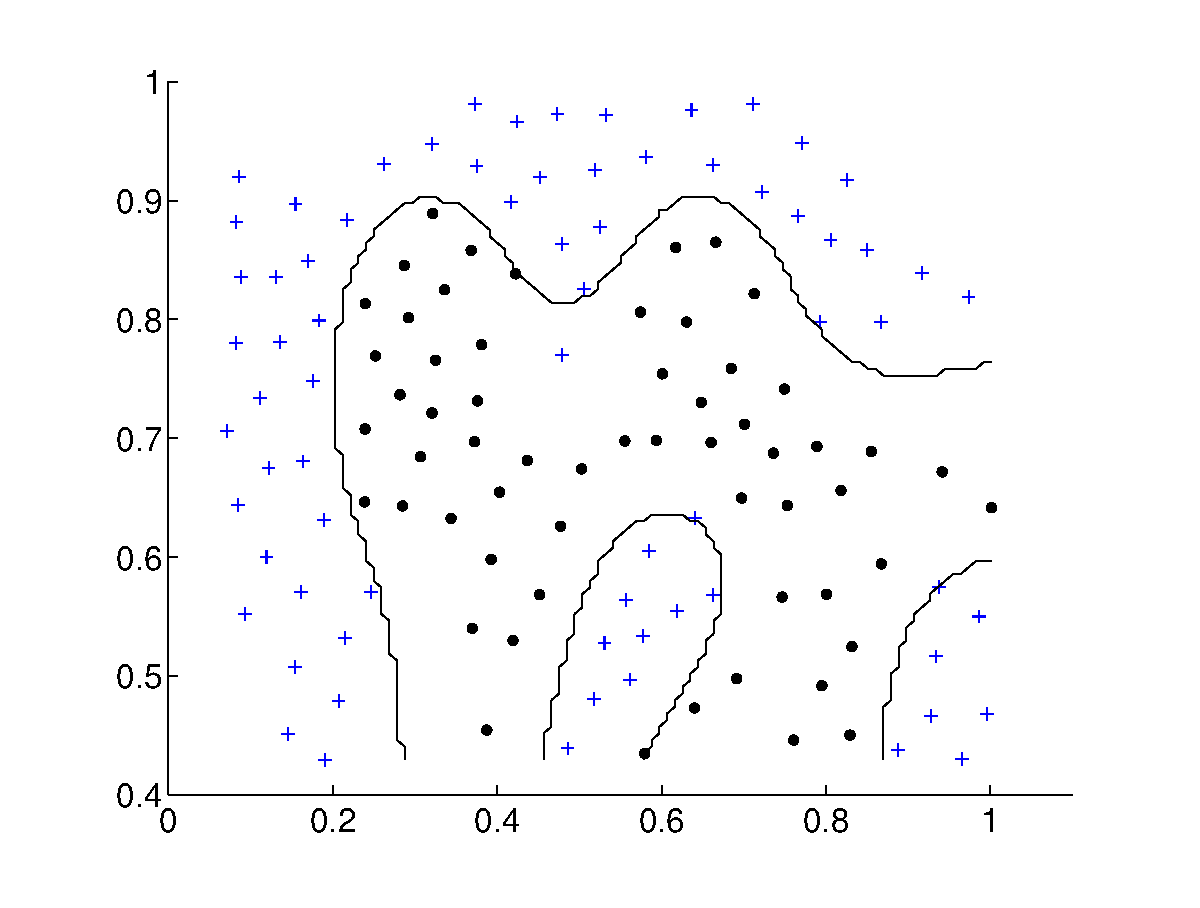
\includegraphics[height=4cm]{a4.eps}
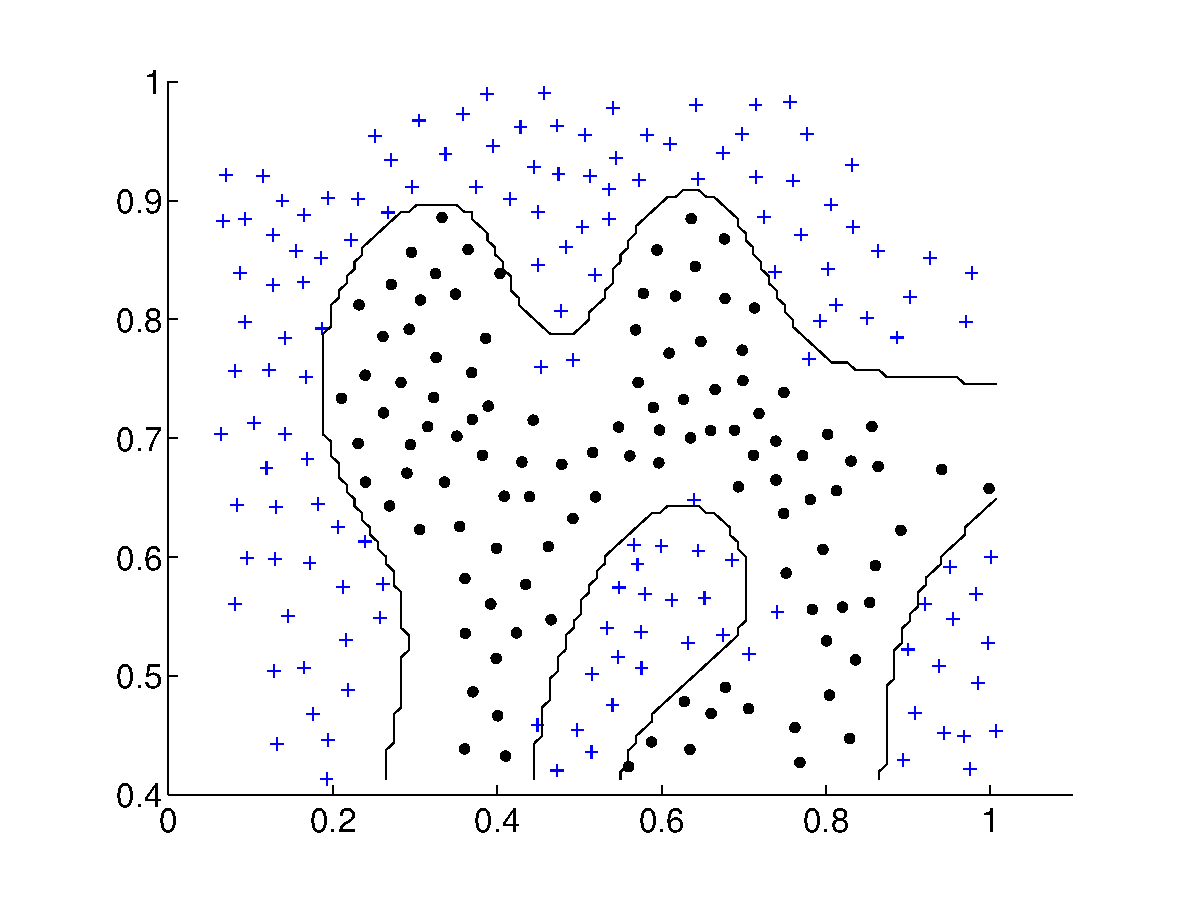
\includegraphics[height=4cm]{a3.eps}
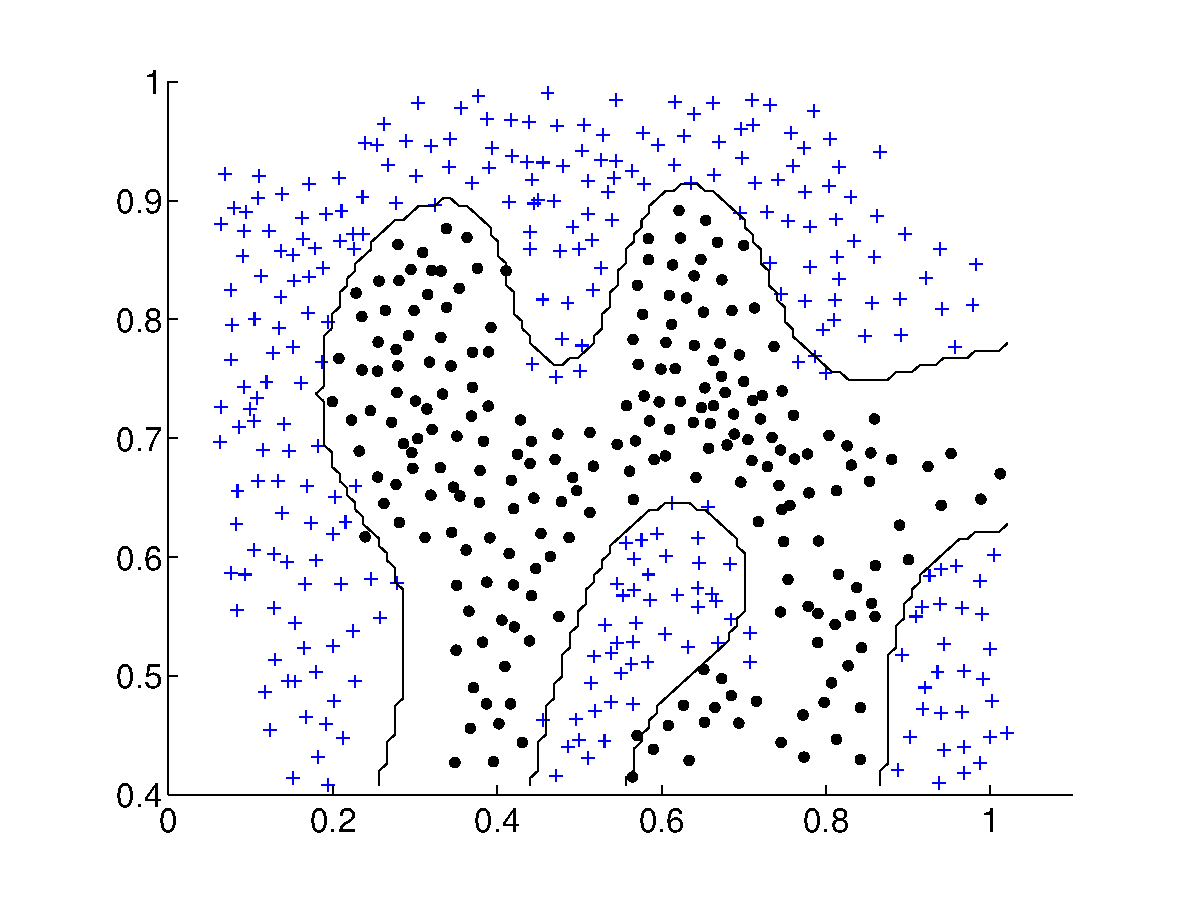
\includegraphics[height=4cm]{a2.eps}

\caption{The 2 pictures in the first row is the result of the first experiment where $k=m$ and $k=0.2m$, 
		and the 2 pictures in the second row is the result of the first experiment where $k=0.1m$ and $k=0.05m$.}
\label{fig:example1}
\end{figure}		
		
		In our second experiment we will use a larger data set: The Skin Segmentation Data Set, which 
		contains much more instances than the previous one. In this experiment we will choose 
		different $k$ ($k=m$,$k=0.1m$, $k=0.01m$ and $k=0.005m$) then 
		we running the $k$-means algorithm to get our new instances individually. After that we got 4 different
		data sets and we use these data sets to train a Gaussian kernel SVM the same as the first experiment
		individually and use the test set to get the 
		accuracy for each SVM. The experiment result was shown in Table 3. As the first experiment, the result 
		is also acceptable. Here we can also choose $k = 0.1 ∗m$ to get the accuracy of 97.25\% which is 
		only 2.22\% lower than the result of the original data set.

\begin{table}[tbp]
\centering  
\begin{tabular}{c|c|c|c|c}
\hline
		the value of $k$ &$k=m$ &$k=0.1*m$ &$k=0.01*m$ &$k=0.005*m$\\ 
\hline  
		accuracy of test set &99.47\% &\textbf{97.25\%} &85.56\% &82.11\%\\    
		 
		training time & 1543.8s &\textbf{7.2s} &0.62s & 0.27s \\
		
		memory requirements & 765.81kb & \textbf{76.59kb} & 7.69kb & 3.84kb \\    
\hline
\end{tabular}
\caption{The result of the second experiment when $k=m, k=0.1m, k=0.01m$ and $k=0.005m$.}
\end{table}


\subsection{Discussion}
		In this paper we provide a method that can alleviate the problem caused by the kernel method when 
		the training instances are too many. We use $k$-means algorithm to divide the training set into $k$ 
		different clusters and label each cluster according to the instances of the cluster. We use kernel 
		SVM to test our algorithm and the result turns to be fairly good. From the Fig.1 we can 
		see that the instance selection process works and it generate a new data set that have a similar 
		distribution with the original data set. In our experiments we 
		choose different $k$ to get different data set, and in both experiment we can get a good result if 
		we choose $k = 0.1 ∗ m$. Generally we can not say that for every data set $k = 0.1 ∗ m$ will 
		always get a good result, because $k$ is influenced by the characters of 
		the data set. Therefore we need to choose different $k$ and use the test set to get the perfomance
		of the corresponding classifier, and as we can 
		see from the result of the experiments, we will lose some of the accuracy if $k$ is lower than $m$, 
		and the smaller the $k$ is the lower the accuracy is. That is easy to explain: during the instance 
		selection we loss some of the information of data set. So one of the most important thing we need to 
		think about when use this method in practice is to make a balance between the lose of accuracy and 
		the size of the new data set.
		
		However there are still two problems need to be solved: the high cost of the $k$-means and how to generate
		good clusters. For the first problem we can solve it by setting a max iteration times instead of 
		repeating until converging. For the second problem we can repeat the $k$-means several times (for example 10 times), 
		and each time select $k$ random instances to initialize the centroids and use the Distortion function\footnote{ 
		In the function $x_n^{(ci)}$ means the centroid for instance $x^{(i)}$.}:
		\[
			D({x^{(1)}},{x^{(2)}},...,{x^{(m)}}) = \sum\limits_{i = 1}^m {{{\left\| {{x^{(i)}} - x_n^{(ci)}} \right\|}^2}} 
		\]
		to compute the total distance between each instance and its centroid, after that select the clusters with the 
		minima value of the distortion function so that we can greatly reduce the possibility of bad clusters.
		
		At last, to generalize our approach we may need to use different distance (in this paper we use 
		Euclidian distance) to calculate the similarity in the $k$-means algorithm and different kernel function 
		for different problem.


\begin{thebibliography}{4}

\bibitem{jour1} Wu, Xindong, et al. "Top 10 algorithms in data mining." 
Knowledge and Information Systems 14.1 (2008): 1-37.

\bibitem{book1}Shawe-Taylor, John, and Nello Cristianini. 
Kernel methods for pattern analysis. Cambridge university press, 2004.

\bibitem{proceeding1}Gretton, Arthur, et al. "A kernel method for the 
two-sample-problem." Advances in neural information processing systems. 2006.

\bibitem{jour2}Brighton, Henry, and Chris Mellish. "Advances in instance 
selection for instance-based learning algorithms." Data mining and knowledge discovery 6.2 (2002): 153-172.

\bibitem{jour3} Aha, David W., Dennis Kibler, and Marc K. Albert. 
"Instance-based learning algorithms." Machine learning 6.1 (1991): 37-66.

\bibitem{proceeding2} Lange, Tilman, and Joachim M. Buhmann. "Fusion of similarity data in clustering." NIPS. 2005.

\bibitem{proceeding3} Zavrel, Jakub, and Walter Daelemans. "Memory-based learning: 
Using similarity for smoothing." Proceedings of the eighth conference on European 
chapter of the Association for Computational Linguistics. Association for Computational Linguistics, 1997.

\end{thebibliography}

\end{document}
